\documentclass[12pt]{article}
\usepackage{latexsym,amssymb,amsmath} % for \Box, \mathbb, split, etc.
% \usepackage[]{showkeys} % shows label names
\usepackage{cite} % sorts citation numbers appropriately
\usepackage{path}
\usepackage{url}
\usepackage{verbatim}
\usepackage{float}
\usepackage{subfig}
\usepackage[pdftex]{graphicx}
\usepackage{pdfpages}


\usepackage{hyperref}

\usepackage{xcolor}
\hypersetup{
	colorlinks,
	linkcolor={red!50!black},
	citecolor={blue!50!black},
	urlcolor={blue!80!black}
}



% horizontal margins: 1.0 + 6.5 + 1.0 = 8.5
\setlength{\oddsidemargin}{0.0in}
\setlength{\textwidth}{6.5in}
% vertical margins: 1.0 + 9.0 + 1.0 = 11.0
\setlength{\topmargin}{0.0in}
\setlength{\headheight}{12pt}
\setlength{\headsep}{13pt}
\setlength{\textheight}{625pt}
\setlength{\footskip}{24pt}

\renewcommand{\textfraction}{0.10}
\renewcommand{\topfraction}{0.85}
\renewcommand{\bottomfraction}{0.85}
\renewcommand{\floatpagefraction}{0.90}

\makeatletter
\setlength{\arraycolsep}{2\p@} % make spaces around "=" in eqnarray smaller
\makeatother

% change equation, table, figure numbers to be counted inside a section:
\numberwithin{equation}{section}
\numberwithin{table}{section}
\numberwithin{figure}{section}

% begin of personal macros
\newcommand{\half}{{\textstyle \frac{1}{2}}}
\newcommand{\eps}{\varepsilon}
\newcommand{\myth}{\vartheta}
\newcommand{\myphi}{\varphi}

\newcommand{\IN}{\mathbb{N}}
\newcommand{\IZ}{\mathbb{Z}}
\newcommand{\IQ}{\mathbb{Q}}
\newcommand{\IR}{\mathbb{R}}
\newcommand{\IC}{\mathbb{C}}
\newcommand{\Real}[1]{\mathrm{Re}\left({#1}\right)}
\newcommand{\Imag}[1]{\mathrm{Im}\left({#1}\right)}

\newcommand{\norm}[2]{\|{#1}\|_{{}_{#2}}}
\newcommand{\abs}[1]{\left|{#1}\right|}
\newcommand{\ip}[2]{\left\langle {#1}, {#2} \right\rangle}
\newcommand{\der}[2]{\frac{\partial {#1}}{\partial {#2}}}
\newcommand{\dder}[2]{\frac{\partial^2 {#1}}{\partial {#2}^2}}

\newcommand{\nn}{\mathbf{n}}
\newcommand{\xx}{\mathbf{x}}
\newcommand{\uu}{\mathbf{u}}

\newcommand{\junk}[1]{{}}

% set two lengths for the includegraphics commands used to import the plots:
\newlength{\fwtwo} \setlength{\fwtwo}{0.45\textwidth}
% end of personal macros


\pdfcompresslevel=9
\pdfminorversion=5
\pdfobjcompresslevel=2



\begin{document}
\DeclareGraphicsExtensions{.jpg}

\begin{center}
\textbf{\Large An Overview of Deep Residual Neural Networks\newline(ResNets)} \\[6pt]
  Fabio Andres Herrera \\[6pt]
  Escuela de Ingeniería de Sistemas y Computación\\
  Universidad del Valle, Cali - Colombia  \\[6pt]
  fabio.herrera@correounivalle.edu.co
\end{center}

\begin{abstract}

\noindent	
This paper presents an overview of Deep Residual Neural Networks a.k.a (ResNet) based on some recent papers that show the potential of this kind of convolutional neural network (CNN) architecture in different contexts such as machine learning and computer vision domain.

\end{abstract}

\subparagraph{\textit{Key words.}}\textit{ Deep Learning, CNN, ResNets, }


%https://chatbotslife.com/resnets-highwaynets-and-densenets-oh-my-9bb15918ee32

\section{Introduction}

Deep residual networks, or ResNets for short, provided the breakthrough idea of identity mappings in order to enable training of very deep convolutional neural networks. A technique introduced by Microsoft in 2015 allows deeper neural networks to be effectively trained. ResNets won the ImageNet challenge \cite{ILSVRC15} in December with a 3.57\% error score. Recently, researchers have published several papers augmenting the ResNet model with some interesting improvements \cite{He2016}, \cite{Veit2016}, \cite{Wu2017}, \cite{Xie2016} , \cite{Zagoruyko2016}, \cite{Long2016}
, \cite{Huang2016}, \cite{Philipp2017} , \cite{Targ2016} , \cite{Wang2017}. ResNets tweak the mathematical formula for a deep neural network. They tweak the layers’ equations to introduce identity connections between them. The identity function is simply $id(x) = x;$ given an input $x$ it returns the same value $x$ as output. A layer in a traditional neural network learns to calculate a function $y = f(x)$. A residual neural network layer approximately calculates $y = f(x) + id(x) = f(x) + x$. Identity connections enable the layers to learn incremental, or residual, representations. The layers can start as the identity function and gradually transform to be more complex. Such evolution occurs if the parameters for the $f(x)$ part begin at or near \textbf{zero}. The robustness of ResNets has since been proven by various visual recognition tasks and by non-visual tasks involving speech and language\cite{Michael:Online}.

\section{Background} \label{secimport}

Deep Learning is all about neural networks, their background, and concepts.

\subsection{Neural Networks}

\begin{figure}[H] \centering
	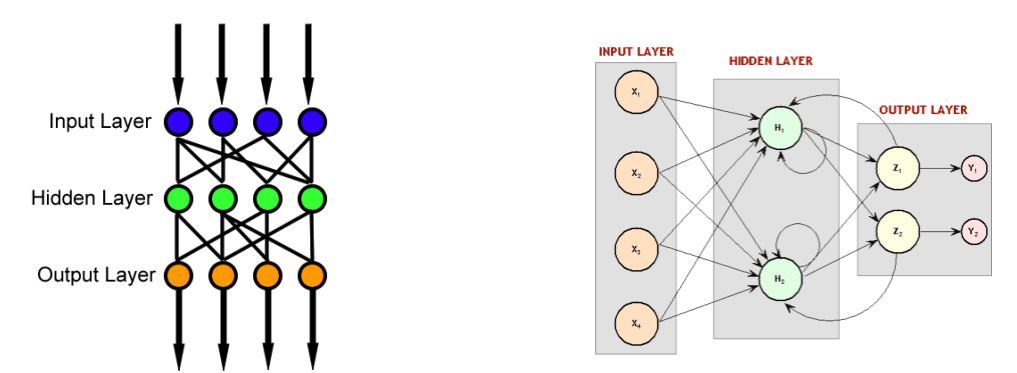
\includegraphics[width=0.9\textwidth]{image7.png}
	\caption{Feed-forward networks (left) and Recurrent neural networks (right) .  Taken from  }
	\label{figre7}
\end{figure}


\subsection{Convolutional Neural Networks (CNN)}

A CNN often consists of convolutional layers, max-pooling layers and fully connected layers. The output of each convolutional layer is a block of 2D images, which are computed by convolving previous feature maps with a small filter. The filter parameters are learned during the training process. The last few layers of CNN are densely connected to each other, and the class scores are obtained from the final layer.


\begin{figure}[H] \centering
	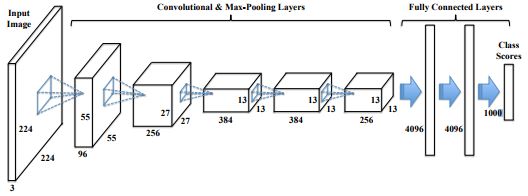
\includegraphics[width=0.9\textwidth]{alexnet.png}
	\caption{Alexnet CNN deep structure}
	\label{alex}
\end{figure}

At Figure \ref{alex} an schematic of a Convolutional Neural network (Alexnet \cite{Krizhevsky2012}). Each layer in this network consists of a set of parameters and neuronal activations. The parameters could be trainable or fixed, depending on the layer. Activations could be non-linear or linear, as described in more detail below. The CNN structure takes a tensor of three-dimensional data as its input, passes it through multiple sets of layers and then outputs a score that represents the semantic class label of the input data. For instance in a simple cat vs. dog classification task, the input could be the image of a kitty and the correct output would be a high score for the cat class. In our application, we feed the CNN with top-view images (with three color channels) from plants. Next we introduce the main layers of a CNN.


\subsection{Convolutional Layer}
This layer is computed by applying multiple filters to the input image, i.e.
sliding the filter window over the entire input image. Different filters can
have different parameters, which lets them detect and learn different image
features. For example, one filter could be in charge of spotting vertical edges,
while another one could detect horizontal edges. The output of this layer is
called a feature map.
Filters are normally designed to be small $(3 × 3, 5 × 5, 7 × 7, . . . )$, to
reduce the number of parameters in the system. As a result, regardless of
the size of the input image, the parameter size remains limited. This is in
contrast to the design of a fully connected neural network where all the units
in the previous layer are connected to every unit in the next layer with unique
parameters, which leads to a sizable parameter set.

\subsection{Max Pooling Layer}
Each feature map obtained from the convolutional layer, is an indicator of
a particular feature in different locations of the input image. We normally
want our descriptors to be robust against minor displacements of the input
data. This is addressed by adding a max pooling layer to the network, which
downsamples the feature maps. In other words, it reduces small patches of
the feature map into single pixels. If a feature is detected anywhere within
the patch, the downsampled patch fires a detection of that feature (local
invariance).
A more practical benefit of the pooling layer is that, reducing the size of
the feature maps leads to a significant decrease in the number of parameters,
which in turn controls overfitting and also speeds up the training process.
Another advantage of pooling layer is that it helps the network to detect
more meaningful and high-level features as it moves on to the deeper layers.
In this structure, the first layer has detected low level features like edges,
whereas the next layer could grab more sophisticated descriptors like leaves
or petiole, and the layer after has learned high-level features that are able to
describe the whole plant.

\subsection{Fully Connected Layer}
After a sequence of multiple convolution and pooling layers, the size of input
data is shrunk dramatically which is suitable as input to a fully connected
(dense) layer. The resulting feature maps up to this point of the network
are vectorized and feed a multi-layer fully connected neural network, whose
last layer (a.k.a classification layer or softmax layer) denotes the scores of
the class labels in our problem.
The last fully connected layer is in charge of computing the scores for each class label. Each neuron in this layer represents a category in the
classification problem, and its class probability can be computed by applying
a softmax function to its inputs from the previous layer.

















%image credit 	http://mesin-belajar.blogspot.com/2016/01/a-brief-history-of-neural-nets-and-deep_84.html




\subsection{Deep Learning}
%https://es.slideshare.net/yuhuang/deep-learning-for-image-denoising-superresolution-27435126






\subsubsection{ Vanishing Gradients }

In some cases some neuron can “die” in the training and become ineffective/useless. This can cause information loss, sometimes very important information.

\subsubsection{ Optimization Difficulty }

If parameters like weights,biases increases due to increasing depth, training the network becomes very difficult. Even this causes in higher training errors.

Hence the problem becomes increasing network depth without affecting from these problems.

One of the biggest advantages of the ResNet is while increasing network depth, it avoids negative outcomes. So we can increase the depth but we have fast training and higher accuracy. Pretty, right?


\subsection{Ensemble learning}
Ensemble methods use multiple learning algorithms to obtain better predictive performance than could be obtained from any of the constituent learning algorithms alone. Unlike a statistical ensemble in statistical mechanics, which is usually infinite, a machine learning ensemble consists of only a concrete finite set of alternative models, but typically allows for much more flexible structure to exist among those alternatives.

An ensemble is itself a supervised learning algorithm, because it can be trained and then used to make predictions. The trained ensemble, therefore, represents a single hypothesis. This hypothesis, however, is not necessarily contained within the hypothesis space of the models from which it is built. Thus, ensembles can be shown to have more flexibility in the functions they can represent. This flexibility can, in theory, enable them to over-fit the training data more than a single model would, but in practice, some ensemble techniques (especially bagging) tend to reduce problems related to over-fitting of the training data.

Empirically, ensembles tend to yield better results when there is a significant diversity among the models.[4][5] Many ensemble methods, therefore, seek to promote diversity among the models they combine.[6][7] Although perhaps non-intuitive, more random algorithms (like random decision trees) can be used to produce a stronger ensemble than very deliberate algorithms (like entropy-reducing decision trees).[8] Using a variety of strong learning algorithms, however, has been shown to be more effective than using techniques that attempt to dumb-down the models in order to promote diversity.[9]

\subsection{Network depth}

Network depth is of crucial importance in neural network architectures, but deeper networks are more difficult to train. The residual learning framework eases the training of these networks, and enables them to be substantially deeper — leading to improved performance in both visual and non-visual tasks. These residual networks are much deeper than their ‘plain’ counterparts, yet they require a similar number of parameters (weights).

\subsection{Residual Learning}

In general, in a deep convolutional neural network, several layers are stacked and are trained to the task at hand. The network learns several low/mid/high level features at the end of its layers. In residual learning, instead of trying to learn some features, we try to learn some residual. Residual can be simply understood as subtraction of feature learned from input of that layer. ResNet does this using shortcut connections (directly connecting input of nth layer to some $(n+x)th$ layer. It has proved that training this form of networks is easier than training simple deep convolutional neural networks and also the problem of degrading accuracy is resolved



\section{Residual Networks} \label{secreferences}

%http://cv-tricks.com/cnn/understand-resnet-alexnet-vgg-inception/

As per what we have seen so far, increasing the depth should increase the accuracy of the network, as long as over-fitting is taken care of. But the problem with increased depth is that the signal required to change the weights, which arises from the end of the network by comparing ground-truth and prediction becomes very small at the earlier layers, because of increased depth. It essentially means that earlier layers are almost negligible learned. This is called vanishing gradient. The second problem with training the deeper networks is, performing the optimization on huge parameter space and therefore naively adding the layers leading to higher training error. Residual networks allow training of such deep networks by constructing the network through modules called residual models as shown in the figure. This is called degradation problem. The intuition around why it works can be seen as follows:


%https://adeshpande3.github.io/adeshpande3.github.io/The-9-Deep-Learning-Papers-You-Need-To-Know-About.html

\subsection{Residual Block}


\begin{figure}[H] \centering
	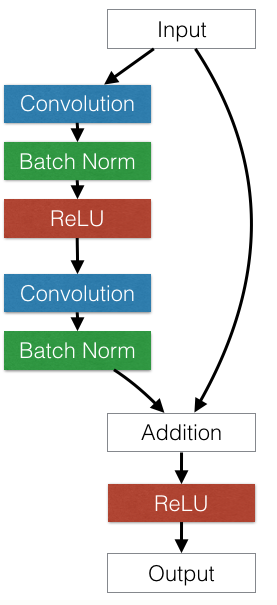
\includegraphics[width=0.2\textwidth]{res1.png}
	\caption{Residual block}
	\label{ree1}
\end{figure}

The idea behind a residual block is that you have your input x go through conv-relu-conv series. This will give you some F(x). That result is then added to the original input x. Let’s call that H(x) = F(x) + x. In traditional CNNs, your H(x) would just be equal to F(x) right? So, instead of just computing that transformation (straight from x to F(x)), we’re computing the term that you have to add, F(x), to your input, x. Basically, the mini module shown below is computing a “delta” or a slight change to the original input x to get a slightly altered representation (When we think of traditional CNNs, we go from x to F(x) which is a completely new representation that doesn’t keep any information about the original x). The authors believe that “it is easier to optimize the residual mapping than to optimize the original, unreferenced mapping”.




%http://neural.vision/blog/article-reviews/deep-learning/he-resnet-2015/

In recent years Deep Convolutional Neural Networks (CNN) demonstrated a high performance on image classification tasks. Experiments showed that the number of layers (depth) in a CNN is correlated to the performance in image recognition tasks.  This led to the idea that deeper networks should perform better. Creating deep networks is not as simple as adding layers. One problem is the vanishing/exploding gradients, which hamper the convergence. This obstacle can be overcome by normalized initialization and intermediate normalization layers, so that networks start converging for stochastic gradient descend (SGD) using the backpropagation algorithm. Another problem is the degradation, if the depth of a network increases, the accuracy gets saturated and then degrades rapidly. (Figure \ref{figre6}) A way to counter the degradation problem is using residual learning. 

\begin{figure}[H] \centering
	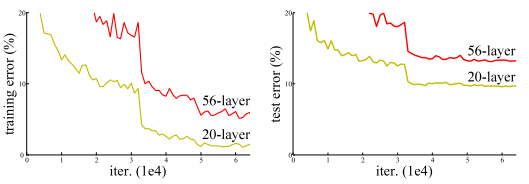
\includegraphics[width=0.6\textwidth]{image6.png}
	\caption{Training error (left) and test error (right) on CIFAR-10 with 20-layer and 56-layer "plain" networks reproduced from XXXX }
	\label{figre6}
\end{figure}


The ResNet technique has shown deeper neural network models can train successfully. The model Microsoft used in ImageNet 2015 has 152 layers. That’s significantly deeper than previous competition winners. Deeper models tend to hit obstacles during the training process. The gradient signal vanishes with increasing network depth. But the identity connections in ResNets propagate the gradient throughout the model.

Researchers have hypothesized that deeper neural networks have more representational power. Deeper nets gain this power from hierarchically composing shallower feature representations into deeper representations. For instance, in face recognition, pixels make edges and edges make corners. Corners define facial features such as eyes, noses, mouths and chins. Facial features compose to define faces.

Which brings me to the first paper, Benefits of depth in neural networks by Matus Telgarsky. This paper shows mathematically that depth is necessary for representational power. It proves it for the class of activation functions common in deep learning research, such as rectified linear units (\textbf{ReLU}). Given a number k, there exist neural networks of depth $O(k^3)$, that are intractable. No depth k neural network can approximate them without exponentially many neurons $Ω(2^k)$. Thus, ResNets will be important to enable complex models of the world.

The second paper I’d like to highlight is Identity Mappings in Deep Residual Networks, by He et al. These are the original authors of the ResNet paper. The original technique only approximated identity connections between layers. Really, the layers still used nonlinear activations after the identity connections. These nonlinearities impede gradient propagation. The new paper runs with the identity connection concept. The signal propagates unchanged throughout the entire network. The activation functions between layers are absent. The new technique improves training and test performance.


\begin{figure} \centering
	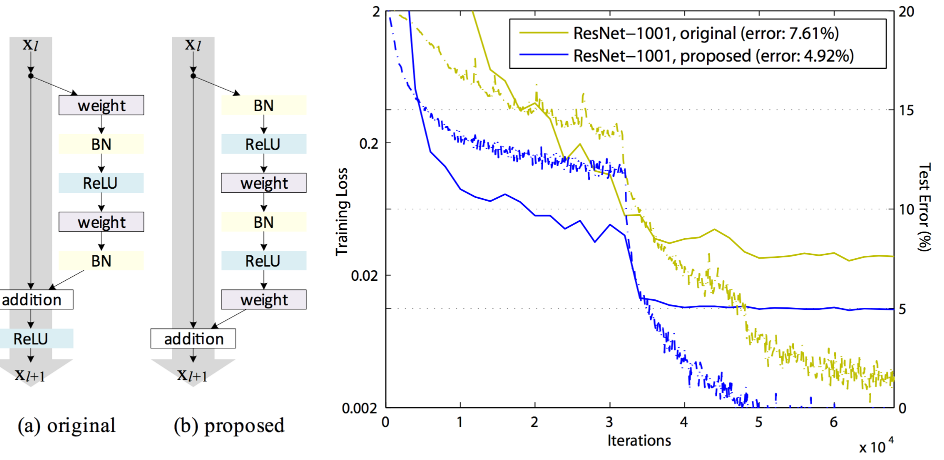
\includegraphics[width=0.9\textwidth]{image1.png}
	\caption{Original versus proposed ResNet unit, and performance.}
	\label{figsolplot}
\end{figure}

The third paper is Resnet in Resnet: Generalizing Residual Architectures, by Targ et al. This paper experiments with additional complexity that runs parallel to the ResNet modules. Essentially, for every ResNet layer, they place a traditional convolutional layer next to it. They allow these parallel layers to exchange information. What results is a fractal ResNet structure. Groups of these modified ResNet modules can coordinate to learn longer-term ResNet structures.


\begin{figure} \centering
	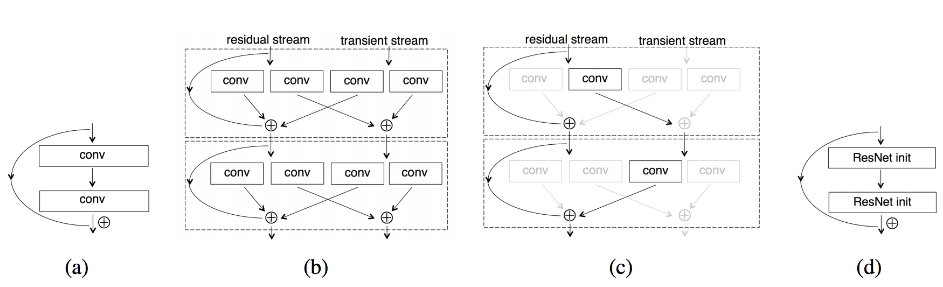
\includegraphics[width=0.9\textwidth]{image2.png}
	\caption{ResNet in ResNet fractal structure.}
	\label{figure2}
\end{figure}


Next, is one of the most interesting papers I’ve seen: Deep Networks with Stochastic Depth, by Huang et al. This paper enables practical training of neural networks with thousands of layers. It modifies the technique dropout to remove layers from the network during training time. Entire layers get dropped at random. The remaining layers must compensate for their missing inputs by relying on lower inputs. Concretely, the technique sets the f(x) component to zero for several random layers, leaving the identity connections. Then the training procedure runs for a single step. Then those layers get reactivated while new ones get zeroed. During training, the depth of the network can be much smaller than normal. This results in fewer calculations and more efficient training throughput. The entire depth of the model is then used at inference time.


\begin{figure} \centering
	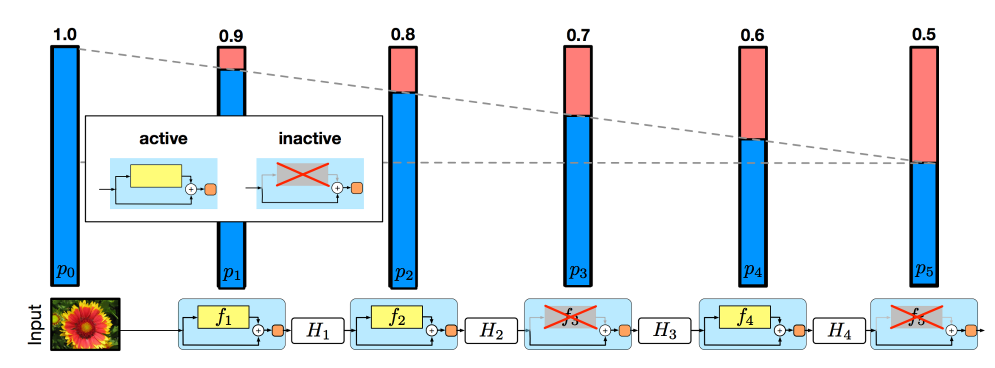
\includegraphics[width=0.9\textwidth]{image3.png}
	\caption{Linear decay of layer dropout probabilities in stochastic depth.}
	\label{figure3}
\end{figure}


Another paper, Bridging the Gaps Between Residual Learning, Recurrent Neural Networks and Visual Cortex by Qianli Liao and Tomaso Poggio, explores the relationship between recurrent nets and residual nets. It augments recurrent nets with identity connections and shows such models have flexible topologies and improved performance. I find the techniques here to be very similar to two other papers: Neural GPUs Learn Algorithms by Łukasz Kaiser and Ilya Sutskever, and Adaptive Computation Time for Recurrent Neural Networks by Alex Graves.

Finally, the paper Deep Residual Networks with Exponential Linear Unit, by Shah et al., combines exponential linear units, an alternative to rectified linear units, with ResNets to show improved performance, even without batch normalization.

\begin{figure} \centering
	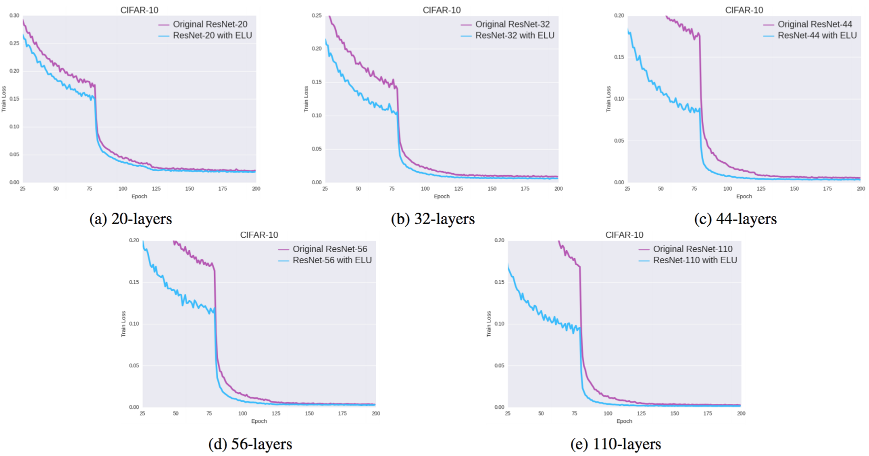
\includegraphics[width=0.9\textwidth]{image4.png}
	\caption{Comparison of the learning behavior of (Auhor model) ant the original ResNet model on CIFAR-10 dataset}
	\label{figure4}
\end{figure}


\subsection{Advantages}

%https://medium.com/@bakiiii/microsoft-presents-deep-residual-networks-d0ebd3fe5887

Some advantages of the ResNet:

\begin{itemize}
	\item To accelerate the speed of training of the deep networks.
	
	\item Instead of widen the network, increasing depth of the network results in less extra parameters.
	
	\item Reducing the effect of Vanishing Gradient Problem.
	
	\item Obtaining higher accuracy in network performance especially in Image Classification.
\end{itemize}



\section{Applications} \label{applications}

The main types of applications of ResNet in computer vision can be categorized as follows:

\begin{itemize}
	\item \textbf{Object Recognition / Classification}: In object recognition, a raw image is given and their task is to identify which class does the image belong to.
	\item \textbf{Classification + Localization}:  If there is only one object in the image, and the task is to find the location of that object, a more specific term given to this problem is the localization problem.
	\item \textbf{Object Detection}: In object detection, the task is to identify where in the image does the objects lies in. These objects might be of the same class or different class altogether.
	\item \textbf{Image Segmentation}: Image Segmentation is a bit sophisticated task, where the objective is to map each pixel to its rightful class.
\end{itemize}




%http://kaiminghe.com/ilsvrc15/ilsvrc2015_deep_residual_learning_kaiminghe.pdf

%http://kaiminghe.com/icml16tutorial/index.html

%http://www.vision.ee.ethz.ch/ntire17/

%https://github.com/KaimingHe/deep-residual-networks#third-party-re-implementations

%\section{Q \& A} \label{qa}



\section{Image classification with pre-trained ResNet model} \label{approach}

In this overview, a couple of pre-trained Residual Network (ResNet) models were used for predict \textbf{60} images from a test dataset of real objects:\\
\newline
\noindent
The pre-trained models used to predict were downloaded from:

\begin{itemize}
	\item[] {\textbf{ResNet pre-trained models: } } \url{http://data.dmlc.ml/mxnet/models/imagenet/resnet/}
\end{itemize}

\noindent
Selected pre-trained models were:

\begin{itemize}
\item ResNet-101
\item ResNet-152
\item ResNet-200
\end{itemize}

\noindent
The ResNet used in this overview was implemented in pyhon using an open-source deep learning framework called Apache MXNet \cite{mxnet}.\\\\
\noindent
Prediction results for test images using each implemented ResNet pre-trained model are available in the following Jupyter Notebooks. 

\begin{itemize}
	\item {\textbf{RESNET 101 Layers:} } \url{https://github.com/AndresHerrera/Proyecto_PatternRecognition/blob/master/JupyterNotebook/Predict_RESNET_101.ipynb}
	
	\item {\textbf{RESNET 152 Layers:} } \url{https://github.com/AndresHerrera/Proyecto_PatternRecognition/blob/master/JupyterNotebook/Predict_RESNET_152.ipynb}
	
	\item {\textbf{RESNET 200 Layers:} } \url{https://github.com/AndresHerrera/Proyecto_PatternRecognition/blob/master/JupyterNotebook/Predict_RESNET_200.ipynb}	
\end{itemize}





\section{Conclusions}

Deeper neural networks are more difficult to train \cite{Zagoruyko2016}, residual networks can be viewed as a collection of many paths, instead of a single ultra deep network. When increasing the depth of traditional networks, there is an initial increase in accuracy, then it plateaus, and then, if the depth is further increased, the accuracy will rapidly fall off. The training error also increases with increasing depth and the validation error also increases.



\section*{Acknowledgments}

To Maria Trujillo Ph.D., a teacher in the course Introduction to Pattern Recognition for Computer Vision for its valuable training along the term fall 2017.
 
%\appendix


\bibliographystyle{siam}
\bibliography{template}

\newpage

\section*{Annexes}
\thispagestyle{empty}
\subsection{Deep Residual Network (ResNET-101)}
%\vspace{-8px}
\begin{figure}[H] \centering
	\caption{ResNet 101 - 60 objects dataset, predicting results.}
	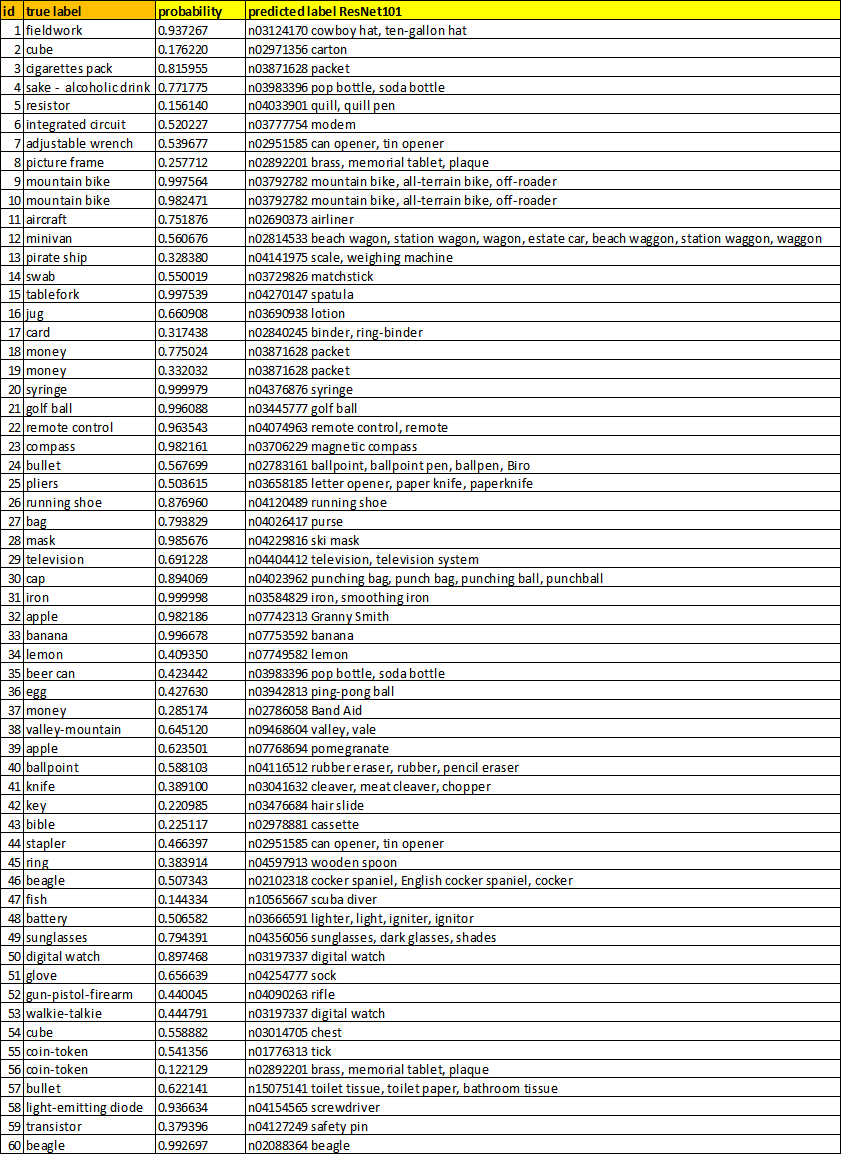
\includegraphics[width=0.9\textwidth]{resnet101.png}
	\label{r1}
\end{figure}
\includepdf[pages={1-},scale=1]{PRINT_Predict_RESNET_101.pdf}

\subsection{Deep Residual Networks (ResNET-152)}
\begin{figure}[H] \centering
	\caption{ResNet 152 - 60 objects dataset, predicting results.}
	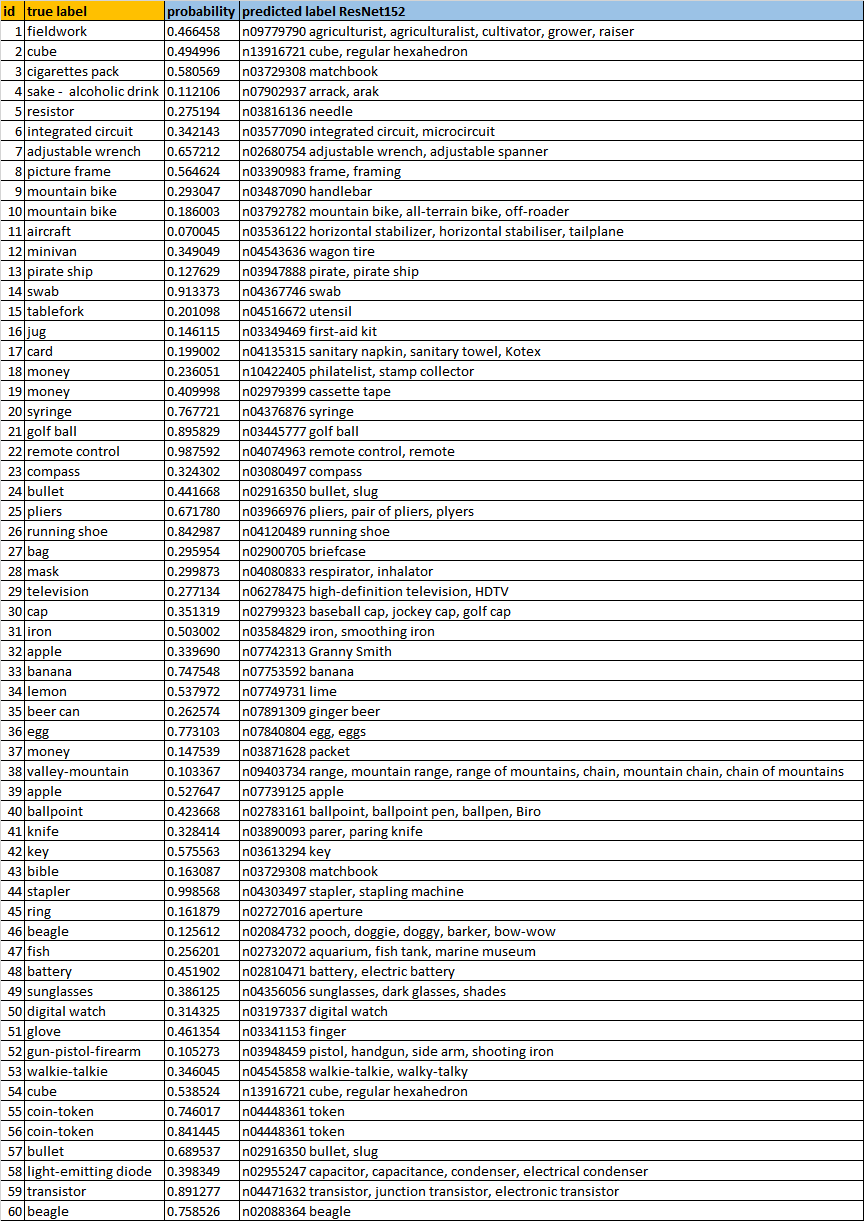
\includegraphics[width=0.9\textwidth]{resnet152.png}
	\label{r2}
\end{figure}
\includepdf[pages={1-},scale=0.75]{PRINT_Predict_RESNET_152.pdf}


\subsection{Deep Residual Network (ResNET-200)}
\begin{figure}[H] \centering
	\caption{ResNet 200 - 60 objects dataset, predicting results.}
	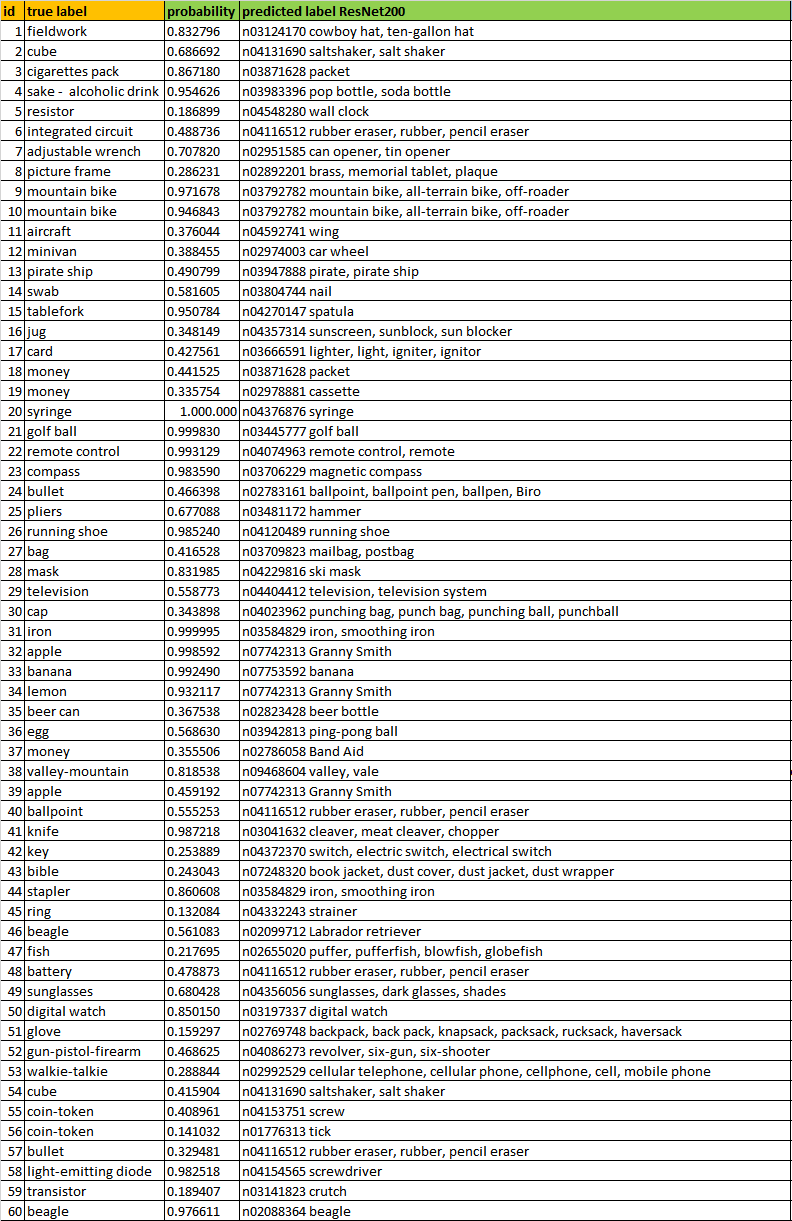
\includegraphics[width=0.9\textwidth]{resnet200.png}
	\label{r3}
\end{figure}
\includepdf[pages={1-},scale=0.75]{PRINT_Predict_RESNET_200.pdf}


\subsection{Network In Network (NIN)}
\begin{figure}[H] \centering
	\caption{NIN - 60 objects dataset, predicting results.}
	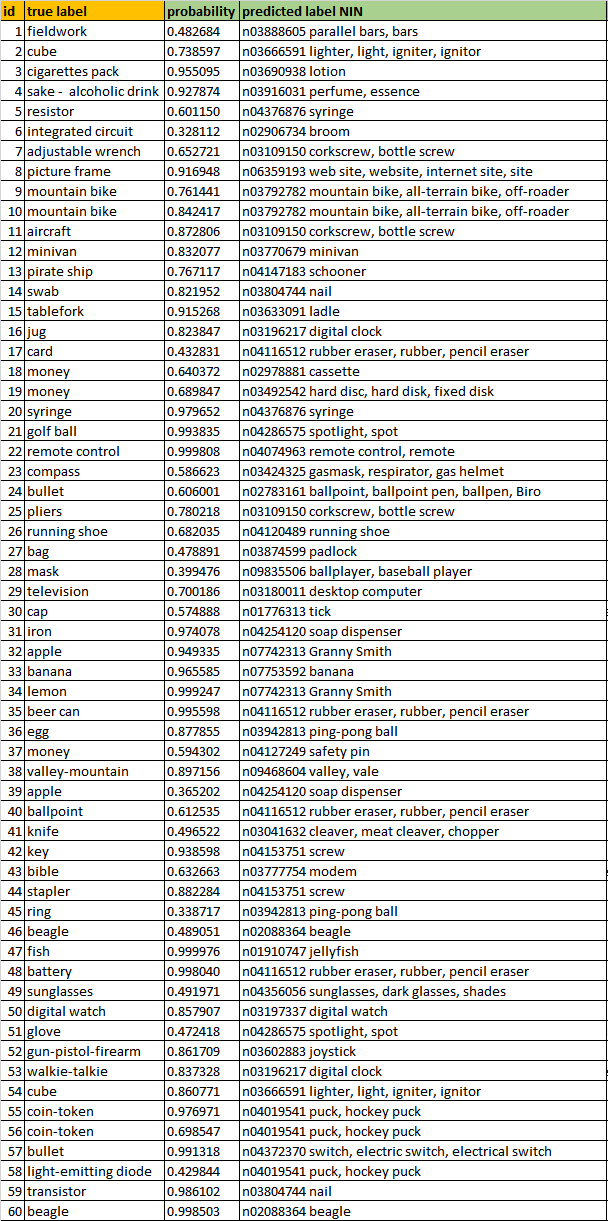
\includegraphics[width=0.9\textwidth]{nin.png}
	\label{r4}
\end{figure}
\includepdf[pages={1-},scale=0.75]{PRINT_Predict_NIN.pdf}




\end{document}

